%%%%%%%%%%%%%%%%%%%%%%%%%%%%% Define Article %%%%%%%%%%%%%%%%%%%%%%%%%%%%%%%%%%
\documentclass{article}
%%%%%%%%%%%%%%%%%%%%%%%%%%%%%%%%%%%%%%%%%%%%%%%%%%%%%%%%%%%%%%%%%%%%%%%%%%%%%%%

%%%%%%%%%%%%%%%%%%%%%%%%%%%%% Using Packages %%%%%%%%%%%%%%%%%%%%%%%%%%%%%%%%%%
\usepackage{geometry}
\usepackage{graphicx}
\usepackage{amssymb}
\usepackage{amsmath}
\usepackage{amsthm}
\usepackage{empheq}
\usepackage{mdframed}
\usepackage{booktabs}
\usepackage{lipsum}
\usepackage{graphicx}
\usepackage{color}
\usepackage{psfrag}
\usepackage{pgfplots}
\usepackage{bm}
%%%%%%%%%%%%%%%%%%%%%%%%%%%%%%%%%%%%%%%%%%%%%%%%%%%%%%%%%%%%%%%%%%%%%%%%%%%%%%%

% Other Settings

%%%%%%%%%%%%%%%%%%%%%%%%%% Page Setting %%%%%%%%%%%%%%%%%%%%%%%%%%%%%%%%%%%%%%%
\geometry{a4paper}

%%%%%%%%%%%%%%%%%%%%%%%%%% Define some useful colors %%%%%%%%%%%%%%%%%%%%%%%%%%
\definecolor{ocre}{RGB}{243,102,25}
\definecolor{mygray}{RGB}{243,243,244}
\definecolor{deepGreen}{RGB}{26,111,0}
\definecolor{shallowGreen}{RGB}{235,255,255}
\definecolor{deepBlue}{RGB}{61,124,222}
\definecolor{shallowBlue}{RGB}{235,249,255}
%%%%%%%%%%%%%%%%%%%%%%%%%%%%%%%%%%%%%%%%%%%%%%%%%%%%%%%%%%%%%%%%%%%%%%%%%%%%%%%

%%%%%%%%%%%%%%%%%%%%%%%%%% Define an orangebox command %%%%%%%%%%%%%%%%%%%%%%%%
\newcommand\orangebox[1]{\fcolorbox{ocre}{mygray}{\hspace{1em}#1\hspace{1em}}}
%%%%%%%%%%%%%%%%%%%%%%%%%%%%%%%%%%%%%%%%%%%%%%%%%%%%%%%%%%%%%%%%%%%%%%%%%%%%%%%

%%%%%%%%%%%%%%%%%%%%%%%%%%%% English Environments %%%%%%%%%%%%%%%%%%%%%%%%%%%%%
\newtheoremstyle{mytheoremstyle}{3pt}{3pt}{\normalfont}{0cm}{\rmfamily\bfseries}{}{1em}{{\color{black}\thmname{#1}~\thmnumber{#2}}\thmnote{\,--\,#3}}
\newtheoremstyle{myproblemstyle}{3pt}{3pt}{\normalfont}{0cm}{\rmfamily\bfseries}{}{1em}{{\color{black}\thmname{#1}~\thmnumber{#2}}\thmnote{\,--\,#3}}
\theoremstyle{mytheoremstyle}
\newmdtheoremenv[linewidth=1pt,backgroundcolor=shallowGreen,linecolor=deepGreen,leftmargin=0pt,innerleftmargin=20pt,innerrightmargin=20pt,]{theorem}{Theorem}[section]
\theoremstyle{mytheoremstyle}
\newmdtheoremenv[linewidth=1pt,backgroundcolor=shallowBlue,linecolor=deepBlue,leftmargin=0pt,innerleftmargin=20pt,innerrightmargin=20pt,]{definition}{Definition}[section]
\theoremstyle{myproblemstyle}
\newmdtheoremenv[linecolor=black,leftmargin=0pt,innerleftmargin=10pt,innerrightmargin=10pt,]{problem}{Problem}[section]
%%%%%%%%%%%%%%%%%%%%%%%%%%%%%%%%%%%%%%%%%%%%%%%%%%%%%%%%%%%%%%%%%%%%%%%%%%%%%%%

%%%%%%%%%%%%%%%%%%%%%%%%%%%%%%% Plotting Settings %%%%%%%%%%%%%%%%%%%%%%%%%%%%%
\usepgfplotslibrary{colorbrewer}
\pgfplotsset{width=8cm,compat=1.9}
%%%%%%%%%%%%%%%%%%%%%%%%%%%%%%%%%%%%%%%%%%%%%%%%%%%%%%%%%%%%%%%%%%%%%%%%%%%%%%%

%%%%%%%%%%%%%%%%%%%%%%%%%%%%%%% Title & Author %%%%%%%%%%%%%%%%%%%%%%%%%%%%%%%%
\title{Title}
\author{Haoyun Qin}
%%%%%%%%%%%%%%%%%%%%%%%%%%%%%%%%%%%%%%%%%%%%%%%%%%%%%%%%%%%%%%%%%%%%%%%%%%%%%%%

\begin{document}
    \maketitle
    \section*{Section 6.3}
    \subsection*{Exercise 43}
    Find a formula for the number of circular \(r\)-permutations of \(n\) people.
    \subsubsection*{Solution}
    We can see that for normal table, the \(r\) - permutations of \(n\) people will be \(^rP_n\) but in circular
    will be different because in the circular, there will be some cases that will be the same with each other if we rotate
    the circle. \\ 
    \begin{center}
        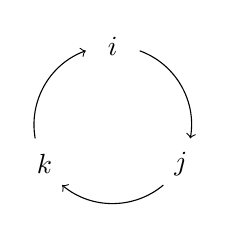
\begin{tikzpicture}[->,scale = 1]
            \node (i) at (90:1cm)  {$i$};
            \node (j) at (-30:1cm) {$j$};
            \node (k) at (210:1cm) {$k$};
        
            \draw (70:1cm)  arc (70:-10:1cm);
            \draw (-50:1cm) arc (-50:-130:1cm);
            \draw (190:1cm) arc (190:110:1cm);
        \end{tikzpicture}
        \space
        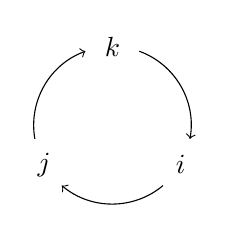
\begin{tikzpicture}[->,scale = 1]
            \node (i) at (90:1cm)  {$k$};
            \node (j) at (-30:1cm) {$i$};
            \node (k) at (210:1cm) {$j$};
        
            \draw (70:1cm)  arc (70:-10:1cm);
            \draw (-50:1cm) arc (-50:-130:1cm);
            \draw (190:1cm) arc (190:110:1cm);
        \end{tikzpicture}
        \space
        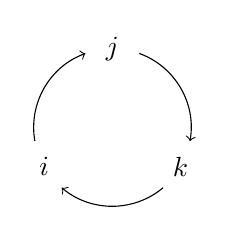
\begin{tikzpicture}[->,scale = 1]
            \node (i) at (90:1cm)  {$j$};
            \node (j) at (-30:1cm) {$k$};
            \node (k) at (210:1cm) {$i$};
        
            \draw (70:1cm)  arc (70:-10:1cm);
            \draw (-50:1cm) arc (-50:-130:1cm);
            \draw (190:1cm) arc (190:110:1cm);
        \end{tikzpicture}
    \end{center}
    For example, let take \(n = 3\) and we will need to find the 3 - permutations of 3 people. Basically, we will calculate by
    \(3! = 6\). However, on the picture above, we can see that there are 3 permutations but these permutations are the same
    because by rotating the circle, we will get second and the third from the first one. If we write all of the permutation as usual on
    the circular, it will be: \\ 
    \begin{center}
        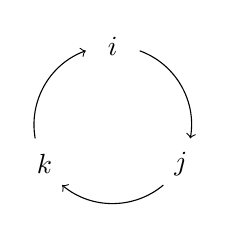
\begin{tikzpicture}[->,scale = 1]
            \node (i) at (90:1cm)  {$i$};
            \node (j) at (-30:1cm) {$j$};
            \node (k) at (210:1cm) {$k$};
        
            \draw (70:1cm)  arc (70:-10:1cm);
            \draw (-50:1cm) arc (-50:-130:1cm);
            \draw (190:1cm) arc (190:110:1cm);
        \end{tikzpicture}
        \space
        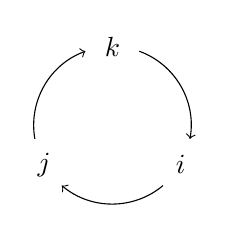
\begin{tikzpicture}[->,scale = 1]
            \node (i) at (90:1cm)  {$k$};
            \node (j) at (-30:1cm) {$i$};
            \node (k) at (210:1cm) {$j$};
        
            \draw (70:1cm)  arc (70:-10:1cm);
            \draw (-50:1cm) arc (-50:-130:1cm);
            \draw (190:1cm) arc (190:110:1cm);
        \end{tikzpicture}
        \space
        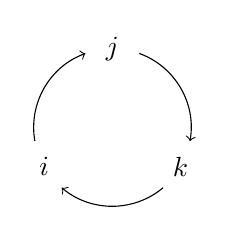
\begin{tikzpicture}[->,scale = 1]
            \node (i) at (90:1cm)  {$j$};
            \node (j) at (-30:1cm) {$k$};
            \node (k) at (210:1cm) {$i$};
        
            \draw (70:1cm)  arc (70:-10:1cm);
            \draw (-50:1cm) arc (-50:-130:1cm);
            \draw (190:1cm) arc (190:110:1cm);
        \end{tikzpicture}
        
        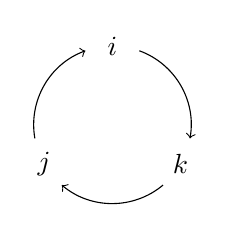
\begin{tikzpicture}[->,scale = 1]
            \node (i) at (90:1cm)  {$i$};
            \node (j) at (-30:1cm) {$k$};
            \node (k) at (210:1cm) {$j$};
        
            \draw (70:1cm)  arc (70:-10:1cm);
            \draw (-50:1cm) arc (-50:-130:1cm);
            \draw (190:1cm) arc (190:110:1cm);
        \end{tikzpicture}
        \space
        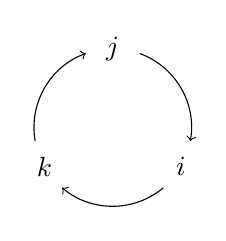
\begin{tikzpicture}[->,scale = 1]
            \node (i) at (90:1cm)  {$j$};
            \node (j) at (-30:1cm) {$i$};
            \node (k) at (210:1cm) {$k$};
        
            \draw (70:1cm)  arc (70:-10:1cm);
            \draw (-50:1cm) arc (-50:-130:1cm);
            \draw (190:1cm) arc (190:110:1cm);
        \end{tikzpicture}
        \space
        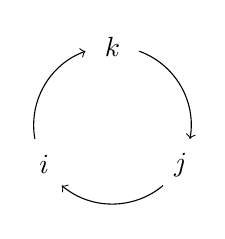
\begin{tikzpicture}[->,scale = 1]
            \node (i) at (90:1cm)  {$k$};
            \node (j) at (-30:1cm) {$j$};
            \node (k) at (210:1cm) {$i$};
        
            \draw (70:1cm)  arc (70:-10:1cm);
            \draw (-50:1cm) arc (-50:-130:1cm);
            \draw (190:1cm) arc (190:110:1cm);
        \end{tikzpicture}
    \end{center}
    Although on the picture show that there are 6 permutations but we just take first one on the first row and the
    second one on the second row. From that observation, we can give out the conclusion that for \(r\) people sitting on the
    table, we will have \(r\) way to rotate the table and we do not want to take the cases when we rotate the table so that
    we can get the formula:
    \begin{align*}
        P_3 = 3! = 6
    \end{align*}
    We do not want to take the rotation cases so that we will divide for the number of people sitting on the table. Because 
    there are 3 people so that we can get that:
    \begin{align*}
        \frac{P_3}{3} = \frac{3!}{3} = \frac{6}{3} = 2
    \end{align*}
    From this observation, we can get the formula when finding the \(n\) - permutations of \(n\) people:
    \begin{align*}
        \frac{P_n}{n} = \frac{n!}{n} = (n-1)!
    \end{align*}
    Moreover, if we are finding the number of circular \(r\)-permutations of \(n\) people. Firstly, we will choose \(r\) people
    from \(n\) people. And then, we will find the permutations of \(r\) people from the above formula. Choosing \(r\) people
    from \(n\) people, we will have that \(^rC_n\) and the permutations of \(r\) people will be \(\frac{r!}{r}\). Multiply them together,
    we will have that:
    \begin{align*}
        ^rC_n \times \frac{r!}{r} = \frac{n!}{r! \times (n - r)!} \times \frac{r!}{r} = \frac{n!}{r \times (n - r)!}
    \end{align*}
    \subsection*{Exercise 42}
    Find the number of circular 3-permutations of 5 people.
    \subsubsection*{Solution}
    Choose 3 from 5 people: \(^3C_5 = \frac{5!}{3! \times (5 - 3)!} = 10\)\\ 
    Permutations of 3 people: \((3 - 1)! = 2! = 2\)\\
    The number of circular 3 - permutations of 5 people: \(10 \times 2 = 20\)
    \subsection*{Exercise 44}
    Find a formula for the number of ways to seat \(r\) of \(n\) people around a circular table, where seatings are considered the same if every person has the same two neighbors without regard to which side these neighbors are sitting on.
    \subsubsection*{Solution}
    Let take the same example of \textbf{Exercise 43} where we find the circular 3 - permutations of 3 people, we will have that:
    \begin{center}
        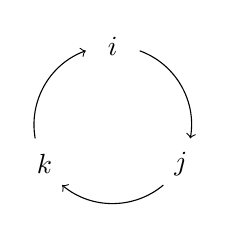
\begin{tikzpicture}[->,scale = 1]
            \node (i) at (90:1cm)  {$i$};
            \node (j) at (-30:1cm) {$j$};
            \node (k) at (210:1cm) {$k$};
        
            \draw (70:1cm)  arc (70:-10:1cm);
            \draw (-50:1cm) arc (-50:-130:1cm);
            \draw (190:1cm) arc (190:110:1cm);
        \end{tikzpicture}
        \space
        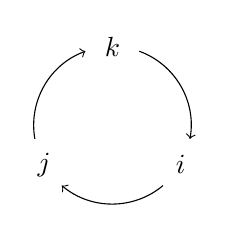
\begin{tikzpicture}[->,scale = 1]
            \node (i) at (90:1cm)  {$k$};
            \node (j) at (-30:1cm) {$i$};
            \node (k) at (210:1cm) {$j$};
        
            \draw (70:1cm)  arc (70:-10:1cm);
            \draw (-50:1cm) arc (-50:-130:1cm);
            \draw (190:1cm) arc (190:110:1cm);
        \end{tikzpicture}
        \space
        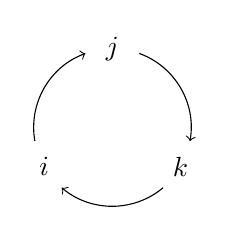
\begin{tikzpicture}[->,scale = 1]
            \node (i) at (90:1cm)  {$j$};
            \node (j) at (-30:1cm) {$k$};
            \node (k) at (210:1cm) {$i$};
        
            \draw (70:1cm)  arc (70:-10:1cm);
            \draw (-50:1cm) arc (-50:-130:1cm);
            \draw (190:1cm) arc (190:110:1cm);
        \end{tikzpicture}
        
        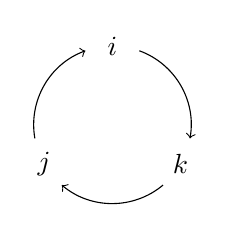
\begin{tikzpicture}[->,scale = 1]
            \node (i) at (90:1cm)  {$i$};
            \node (j) at (-30:1cm) {$k$};
            \node (k) at (210:1cm) {$j$};
        
            \draw (70:1cm)  arc (70:-10:1cm);
            \draw (-50:1cm) arc (-50:-130:1cm);
            \draw (190:1cm) arc (190:110:1cm);
        \end{tikzpicture}
        \space
        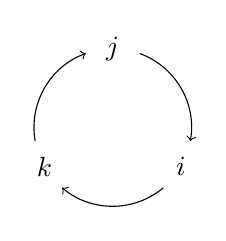
\begin{tikzpicture}[->,scale = 1]
            \node (i) at (90:1cm)  {$j$};
            \node (j) at (-30:1cm) {$i$};
            \node (k) at (210:1cm) {$k$};
        
            \draw (70:1cm)  arc (70:-10:1cm);
            \draw (-50:1cm) arc (-50:-130:1cm);
            \draw (190:1cm) arc (190:110:1cm);
        \end{tikzpicture}
        \space
        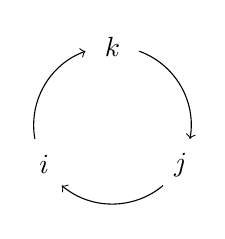
\begin{tikzpicture}[->,scale = 1]
            \node (i) at (90:1cm)  {$k$};
            \node (j) at (-30:1cm) {$j$};
            \node (k) at (210:1cm) {$i$};
        
            \draw (70:1cm)  arc (70:-10:1cm);
            \draw (-50:1cm) arc (-50:-130:1cm);
            \draw (190:1cm) arc (190:110:1cm);
        \end{tikzpicture}
    \end{center}
    In \textbf{Exercise 43}, the first row and the second row are two different permutations. However, on this
    problem requires that the first row and the second row are the same which means that they require the clockwise
    and anti-clockwise cases are all the same. Therefore, in this case, take the formula in \textbf{Exercise 43} and
    then divide by 2 because there are 2 direction clockwise and anti-clockwise and we commit that two of them
    are the same. We have the formula that:
    \begin{align*}
        \frac{P_n}{2 \times n} = \frac{n!}{2 \times n} = \frac{(n - 1)!}{2}
    \end{align*}
    Therefore, the circular \(r\) - permutations of \(n\) people we will first choose \(r\) people from \(n\) people and then
    use the circular \(r\)-permutations of \(n\) people:
    \begin{align*}
        ^rC_k \times \frac{P_n}{2 \times n} = \frac{n!}{r! \times (n - r)!} \times \frac{r!}{2 \times r} = \frac{n!}{2 \times r \times (n -r)!}
    \end{align*}
\end{document}